%%%%%%%%%%%%%%%%%%%%%%%%%%%%%%%%%%%%%%%%%
% Dreuw & Deselaer's Poster
% LaTeX Template
% Version 1.0 (11/04/13)
%
% Created by:
% Philippe Dreuw and Thomas Deselaers
% http://www-i6.informatik.rwth-aachen.de/~dreuw/latexbeamerposter.php
%
% This template has been downloaded from:
% http://www.LaTeXTemplates.com
%
% License:
% CC BY-NC-SA 3.0 (http://creativecommons.org/licenses/by-nc-sa/3.0/)
%
%%%%%%%%%%%%%%%%%%%%%%%%%%%%%%%%%%%%%%%%%

%----------------------------------------------------------------------------------------
%	PACKAGES AND OTHER DOCUMENT CONFIGURATIONS
%----------------------------------------------------------------------------------------

\documentclass[final,hyperref={pdfpagelabels=false}]{beamer}

\usepackage[orientation=portrait,size=a0,scale=1.4]{beamerposter} % Use the beamerposter package for laying out the poster with a portrait orientation and an a0 paper size

\usetheme{I6pd2} % Use the I6pd2 theme supplied with this template

\usepackage[english]{babel} % English language/hyphenation
\usepackage[utf8]{inputenc}

\usepackage{amsmath,amsthm,amssymb,latexsym} % For including math equations, theorems, symbols, etc

%\usepackage{times}\usefonttheme{professionalfonts}  % Uncomment to use Times as the main font
%\usefonttheme[onlymath]{serif} % Uncomment to use a Serif font within math environments

\boldmath % Use bold for everything within the math environment

\usepackage{booktabs} % Top and bottom rules for tables

\graphicspath{{figures/}} % Location of the graphics files

\usecaptiontemplate{\small\structure{\insertcaptionname~\insertcaptionnumber: }\insertcaption} % A fix for figure numbering
\usepackage{url}
%----------------------------------------------------------------------------------------
%	TITLE SECTION 
%----------------------------------------------------------------------------------------

\title{\huge Supervised Classification of Emission Stars Spectra} % Poster title

\author{Jaroslav Vážný, Petr Škoda} % Author(s)

\institute{Astronomical Institute of the Academy of Sciences of the Czech Republic} % Institution(s)

%----------------------------------------------------------------------------------------
%	FOOTER TEXT
%----------------------------------------------------------------------------------------

\newcommand{\leftfoot}{\url{http://physics.muni.cz/~vazny/wiki/index.php}} % Left footer text

\newcommand{\rightfoot}{jaroslav.vazny@gmail.com} % Right footer text

%----------------------------------------------------------------------------------------

\begin{document}

\addtobeamertemplate{block end}{}{\vspace*{2ex}} % White space under blocks

\begin{frame}[t] % The whole poster is enclosed in one beamer frame

\begin{columns}[t] % The whole poster consists of two major columns, each of which can be subdivided further with another \begin{columns} block - the [t] argument aligns each column's content to the top

\begin{column}{.02\textwidth}\end{column} % Empty spacer column

\begin{column}{.465\textwidth} % The first column

%----------------------------------------------------------------------------------------
%	OBJECTIVES
%----------------------------------------------------------------------------------------

\begin{block}{Objectives}

\begin{enumerate}
\item Classify emission star spectra based on H-$\alpha$ line profile.
\item Compare methods for dimensionality reduction.
\item Tune classifier parameters.
\end{enumerate}

\end{block}

%----------------------------------------------------------------------------------------
%	INTRODUCTION
%----------------------------------------------------------------------------------------
            
\begin{block}{Introduction}

\begin{itemize}
\item 
There are 1805 manually classified spectra from Ondřejov observatory divided into 4 categories based on profile of the H-$\alpha$ line. We want to train a SVM classifier to automatically categorize the rest. Figure on the left shows the average spectrum in each category and on the right there are samples of individual spetra.


\end{itemize}

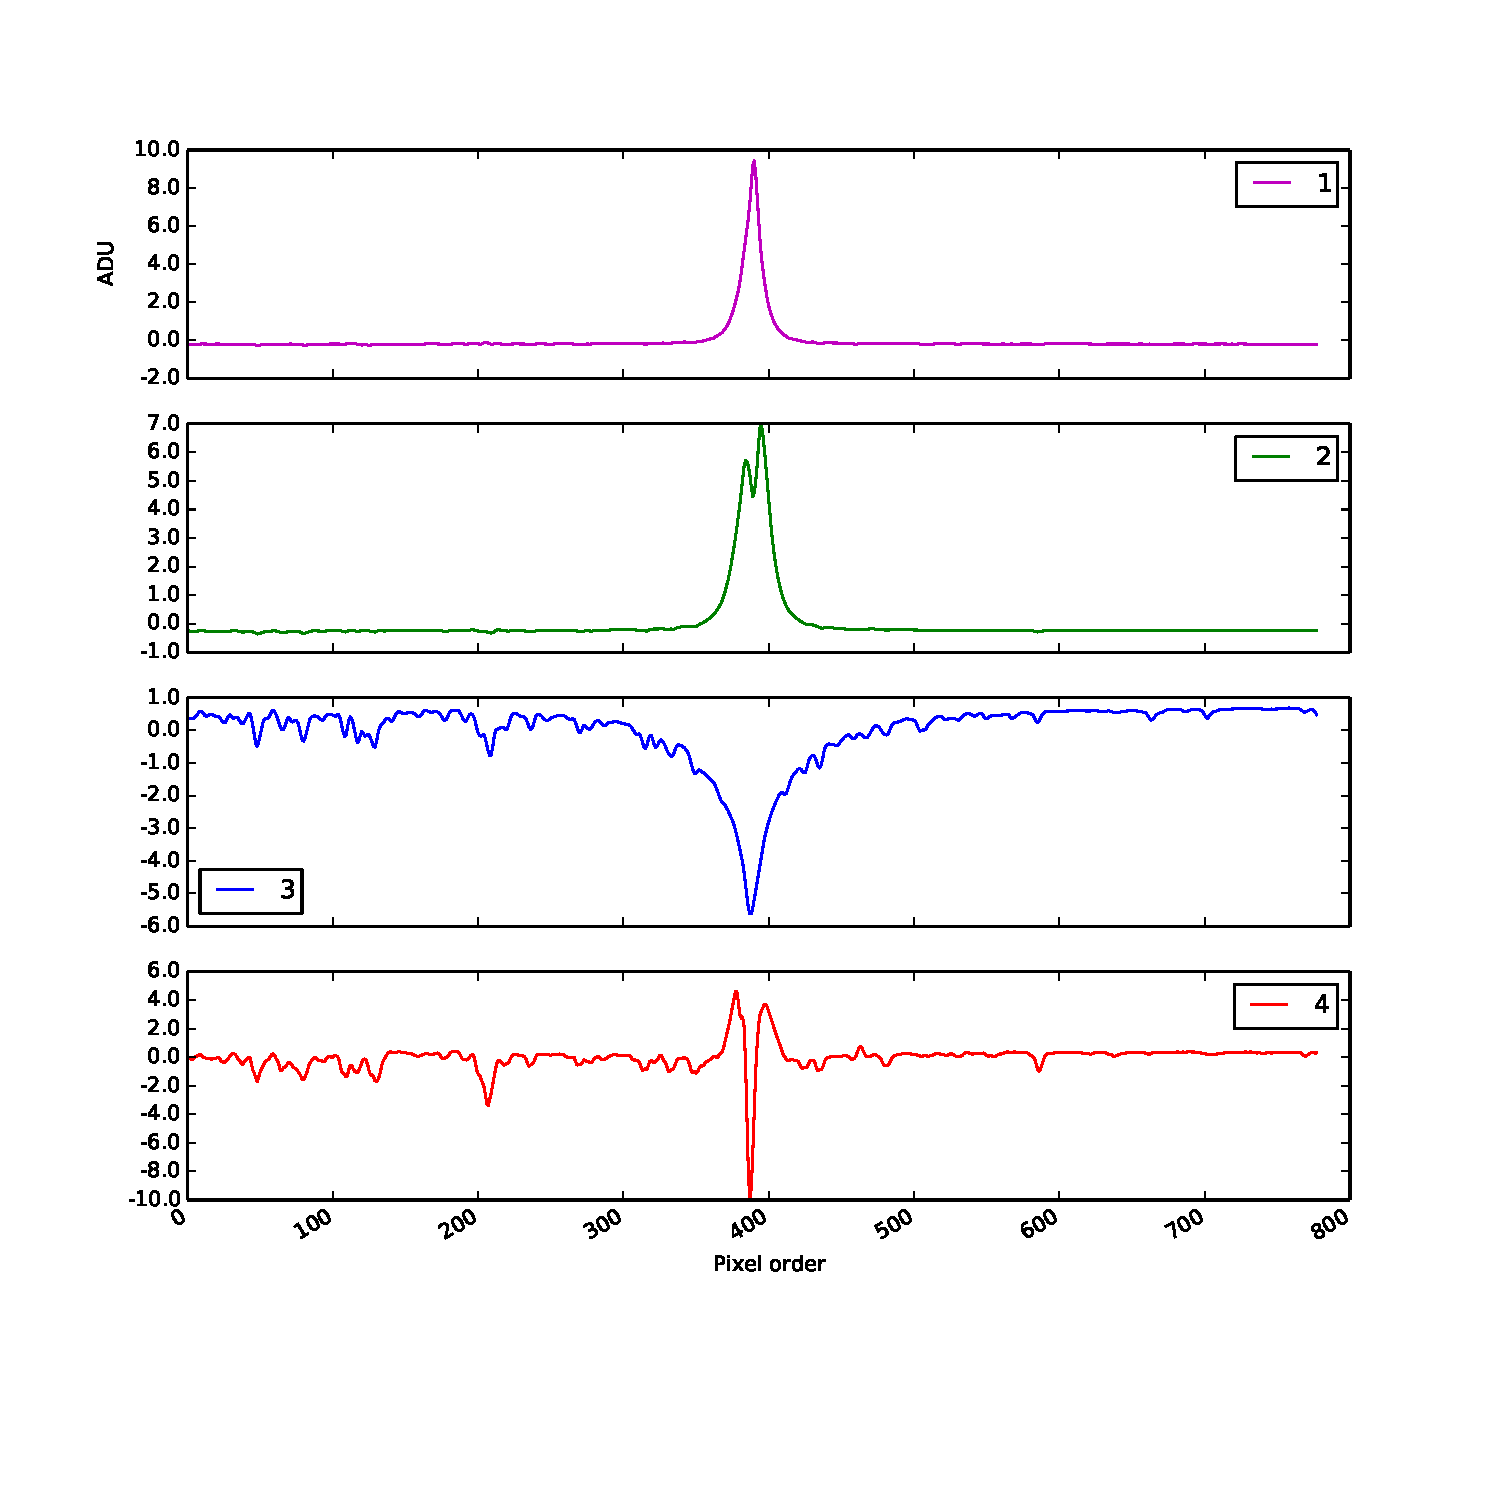
\includegraphics[width=0.45\linewidth]{categories} 
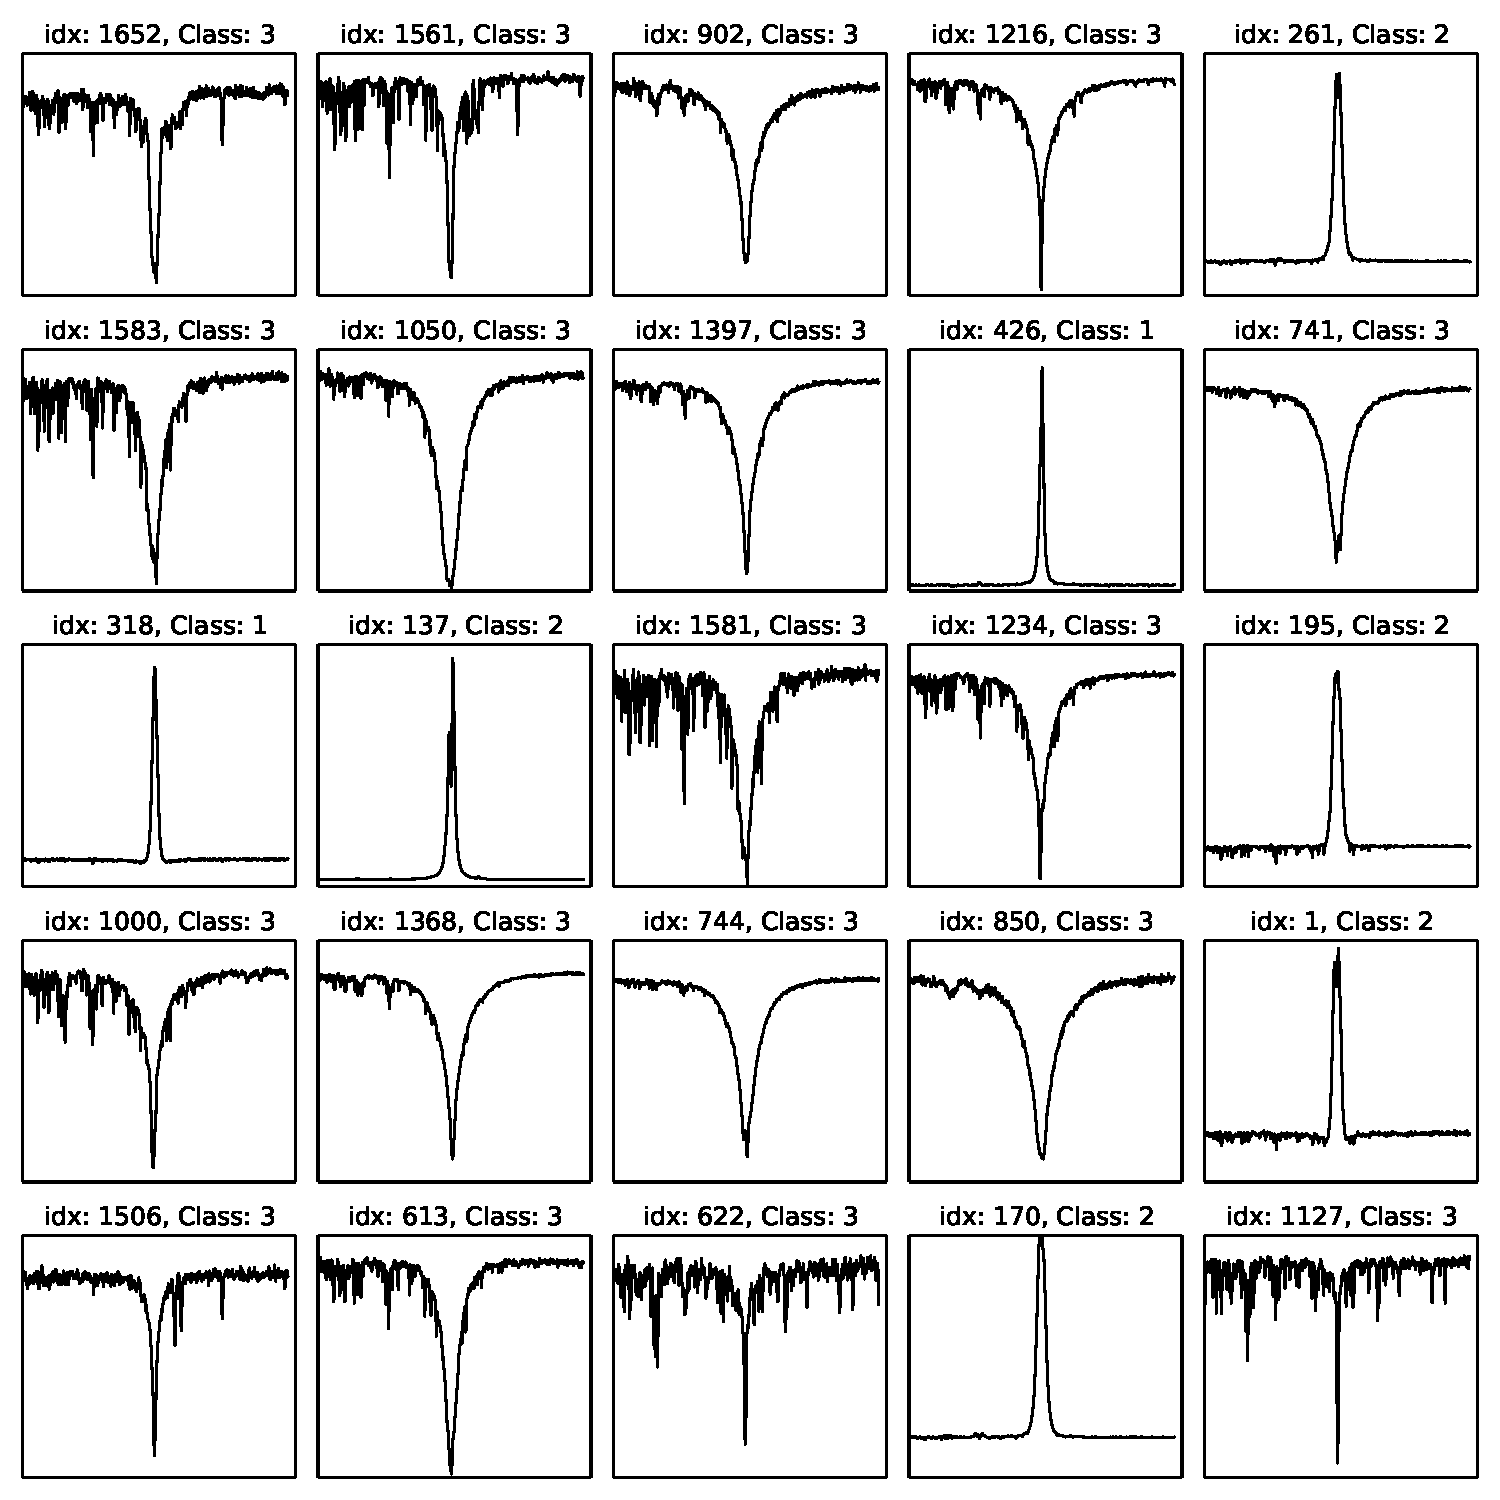
\includegraphics[width=0.45\linewidth]{sample} 

\end{block}

%----------------------------------------------------------------------------------------
%	DIMESNSIONALITY REDUCTION
%----------------------------------------------------------------------------------------

\begin{block}{Dimensionality Reduction}

%\begin{columns} % Subdivide the first main column
%\begin{column}{.54\textwidth} % The first subdivided column within the first main column
\begin{itemize}
\item Each spectrum has 778 points. Different approaches were tested for dimensionlity reduction.
\begin{itemize}
\item PCA: Principal component analysis. Linear dimensionality reduction using Singular Value Decomposition of the data and keeping only the most significant singular vectors to project the data to a lower dimensional space.
\item Isomap: Isometric Mapping. Can be viewed as an extension of Multi-dimensional Scaling (MDS) or Kernel PCA. Isomap seeks a lower-dimensional embedding which maintains geodesic distances between all points.
\item LLE: Locally linear embedding seeks a lower-dimensional projection of the data which preserves distances within local neighborhoods. It can be thought of as a series of local Principal Component Analyses which are globally compared to find the best non-linear embedding. \cite{scikit-learn}
\end{itemize}
%% \item Proin ut vestibulum augue.
%% \begin{itemize}
%% \item Donec dapibus sagittis neque eu ultrices.
%% \end{itemize}
\end{itemize}
%\end{column}

%% \begin{column}{.43\textwidth} % The second subdivided column within the first main column
%% \centering
%% \begin{figure}
%% 
\includegraphics[width=0.8\linewidth]{logo}
%% \caption{Figure caption}
%% \end{figure}
%% \end{column}
%\end{columns} % End of the subdivision

%% \begin{itemize}
%% \item Curabitur sapien ligula, faucibus in feugiat quis, vestibulum a turpis.
%% \begin{itemize}
%% \item Phasellus quis nunc neque. Suspendisse mauris diam, suscipit non gravida in, placerat id enim. Ut nec ipsum in lectus ultrices sagittis.
%% \item Ut nec ipsum in lectus ultrices sagittis.
%% \item Phasellus quis nunc neque.
%% \end{itemize}
%% \end{itemize}

\end{block}

%----------------------------------------------------------------------------------------
%	PARAMETERS TUNING
%----------------------------------------------------------------------------------------

\begin{block}{Parameters tuning}
\begin{columns} % Subdivide the first main column
\begin{column}{.4\textwidth} % The first subdivided column within the first main column
\begin{itemize}
\item Support Vector Machines (SVM) was used as a classifier with Radial Basis Function (RBF) kernal ($\exp(-\gamma |x-x'|^2)$). Grid search was used to 
find optimal values for $C$ and $\gamma$ parameters. There is an example of heatmap for optimal parameters for data reduced by Isomap method. 



\end{itemize}
\end{column}

\begin{column}{.4\textwidth}

%% \begin{table}
%% \begin{tabular}{l l l }
%% \toprule
%% \textbf{Method} & \textbf{C} & \textbf{$\gamma$} \\
%% \midrule
%% PCA & 100 & 0.01 \\
%% ISOMAP & 100 & 1 \\
%% LLE & 100 & 0.1 \\
%% \bottomrule
%% \end{tabular}
%% \caption{ISOMAP Classification report}
%% \end{table}

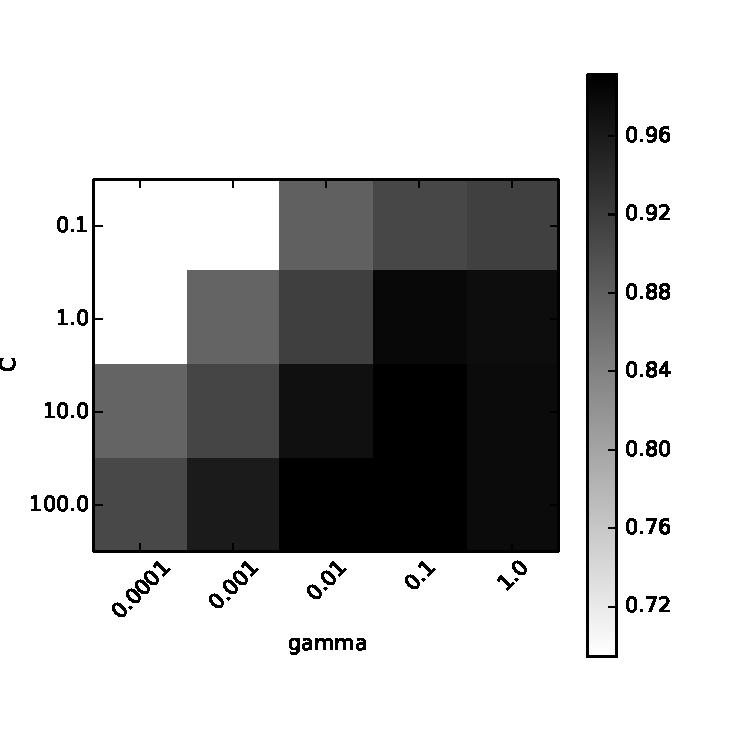
\includegraphics[width=1\linewidth]{tuning_pca}

%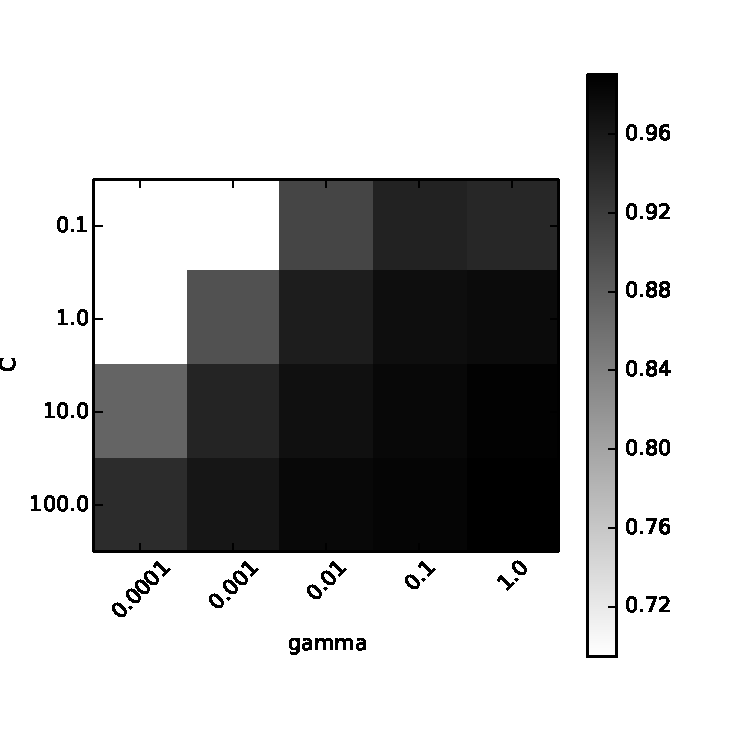
\includegraphics[width=1\linewidth]{tuning_iso}
\end{column}
\end{columns} % End of the subdivision
\end{block}

%----------------------------------------------------------------------------------------
%	CONTACT INFORMATION
%----------------------------------------------------------------------------------------

\setbeamercolor{block title}{fg=black,bg=orange!70} % Change the block title color

\begin{block}{Contact Information}

\begin{itemize}
\item Web: \url{http://physics.muni.cz/~vazny/wiki/index.php}
\item Email: \href{mailto:jaroslav.vazny@gmail.com}{jaroslav.vazny@gmail.com}
\item Phone: +42 606 77 65 64
\end{itemize}

\end{block}

%----------------------------------------------------------------------------------------
%	ACKNOWLEDGEMENTS
%----------------------------------------------------------------------------------------

\begin{block}{Acknowledgment}

\begin{itemize}
\item This research was supported by grant GAČR 13-08195S.
\end{itemize}

\end{block}

%----------------------------------------------------------------------------------------
%	CLASSIFICATION
%----------------------------------------------------------------------------------------

%----------------------------------------------------------------------------------------

\end{column} % End of the first column

\begin{column}{.03\textwidth}\end{column} % Empty spacer column
 
\begin{column}{.465\textwidth} % The second column

%----------------------------------------------------------------------------------------
%	RESULTS
%----------------------------------------------------------------------------------------

\begin{block}{Classification}
\begin{itemize}
\item Data were splited randomly into training (75\%) and testing (25\%) sample. Reports for different reduction aproaches are shown below compared to non-reduced data sample. Precision =  tp / (tp + fp), recall = tp / (tp + fn), f1-score~=~2~*~(precision * recall) / (precision + recall) where tp is true positive, fp false negative and fn false negative.
\end{itemize}

\begin{table}
\begin{tabular}{l l l l l}
\toprule
\textbf{Category} & \textbf{Precision} & \textbf{Recall} & \textbf{f1-score} & \textbf{Support}\\
\midrule
1 &      0.95	&  0.95	 &   0.95 &      61 \\ 
2 &      0.96	&  0.96	 &   0.96 &      74 \\ 
3 &      1.00	&  1.00	 &   1.00 &      303\\ 
4 &      0.93	&  0.93	 &   0.93 &      14 \\ 
\midrule
avg/total   & 0.98   &   0.98  &    0.98  &     452 \\
\bottomrule
\end{tabular}
\caption{Classification report without dimensionality reduction}
\end{table}


\begin{table}
\begin{tabular}{l l l l l}
\toprule
\textbf{Category} & \textbf{Precision} & \textbf{Recall} & \textbf{f1-score} & \textbf{Support}\\
\midrule
1   &    0.89  &   0.95  &   0.92   &    61 \\
2   &    0.96  &   0.91	 &   0.93   &    74 \\
3   &    1.00  &   1.00	 &   1.00   &    303 \\
4   &    1.00  &   0.93	 &   0.96   &    14 \\
\midrule
avg/total   &    0.98  &   0.98 & 0.98 & 452 \\
\bottomrule
\end{tabular}
\caption{ISOMAP Classification report}
\end{table}

\begin{table}
\begin{tabular}{l l l l l}
\toprule
\textbf{Category} & \textbf{Precision} & \textbf{Recall} & \textbf{f1-score} & \textbf{Support}\\
\midrule
        1 &	0.97  &	   1.00	 &    0.98  &	   61\\ 
	2 &	1.00  &	   0.97	 &    0.99  &	   74\\ 
	3 &	0.99  &	   1.00	 &    1.00  &	  303\\ 
	4 &	1.00  &	   0.86	 &    0.92  &	   14\\ 
\midrule
avg/total & 0.99 &     0.99  &    0.99  &     452 \\
\bottomrule
\end{tabular}
\caption{PCA Classification report}
\end{table}

\begin{table}
\begin{tabular}{l l l l l}
\toprule
\textbf{Category} & \textbf{Precision} & \textbf{Recall} & \textbf{f1-score} & \textbf{Support}\\
\midrule
        1  &	0.91  &	   1.00	 &    0.95  &	   61\\ 
	2  &	0.99  &	   0.92	 &    0.95  &	   74\\ 
	3  &	1.00  &	   1.00	 &    1.00  &	  303\\ 
	4  &	0.92  &	   0.86	 &    0.89  &	   14\\ 

\midrule
avg/total & 0.98  &    0.98  &    0.98   &    452 \\
\bottomrule
\end{tabular}
\caption{LLE Classification report}
\end{table}

The left figure shows classification confusion matrix. Graph on the right is a learning curve.


\begin{columns} % Subdivide the first main column
\begin{column}{.4\textwidth} % The first subdivided column within the first main column
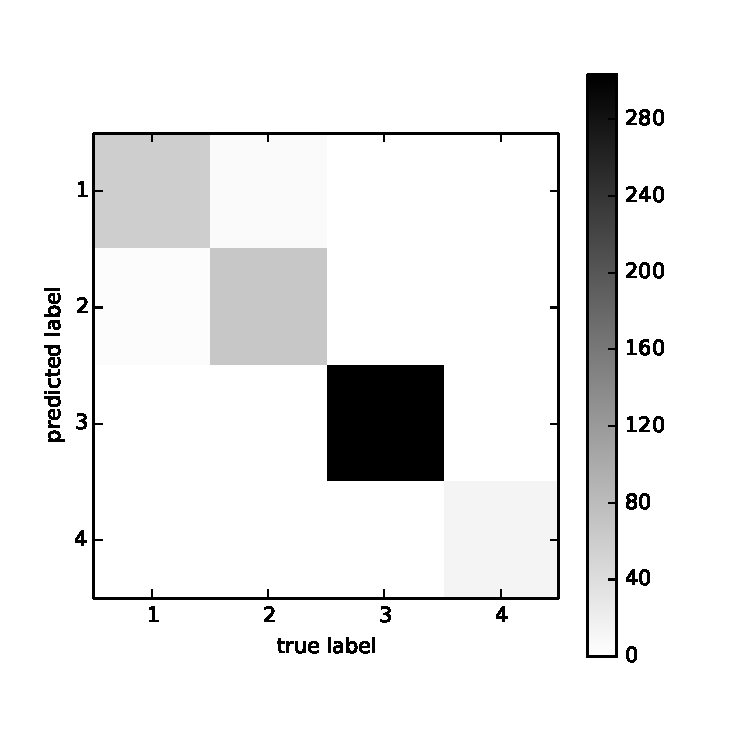
\includegraphics[width=1\linewidth]{confusion}
\end{column}
\begin{column}{.4\textwidth}
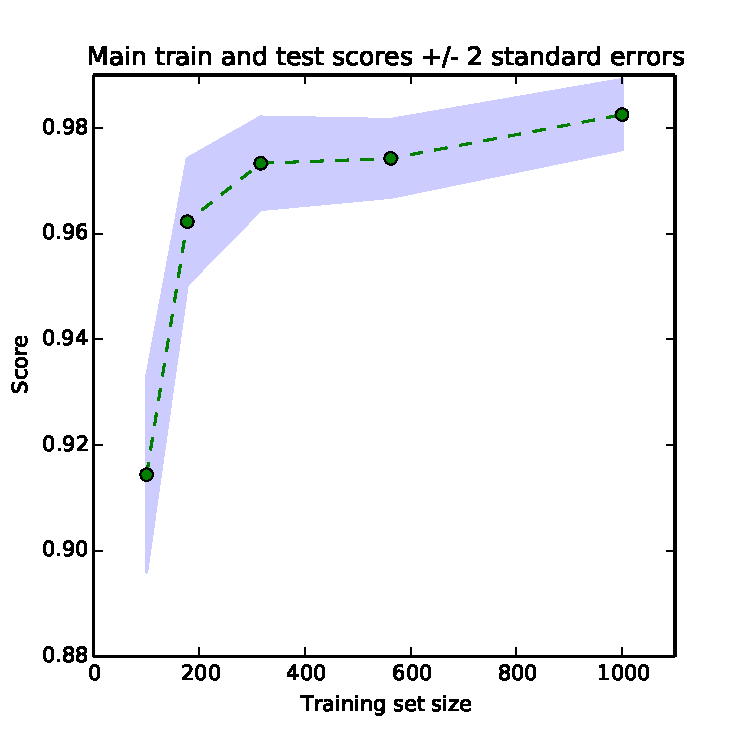
\includegraphics[width=1\linewidth]{learning}
\end{column}
\end{columns} % End of the subdivision
\end{block}


%----------------------------------------------------------------------------------------
%	CONCLUSION
%----------------------------------------------------------------------------------------

\begin{block}{Conclusion}

\begin{itemize}
\item It is possible to dramatically reduce the number of dimensions of spectra in classification problem (here from 778 to 10).
\item PCA, Isomap, LLE and has similar effects in this classification problem.
\item It is always important to tune corresponding hyperparameters.
\end{itemize}

\end{block}

%----------------------------------------------------------------------------------------
%	REFERENCES
%----------------------------------------------------------------------------------------

\begin{block}{References}
        
\nocite{*} % Insert publications even if they are not cited in the poster
\small{\bibliographystyle{unsrt}
\bibliography{reference}}

\end{block}




%----------------------------------------------------------------------------------------

\end{column} % End of the second column

\begin{column}{.015\textwidth}\end{column} % Empty spacer column

\end{columns} % End of all the columns in the poster

\end{frame} % End of the enclosing frame

\end{document}
